
%% bare_conf_compsoc.tex
%% V1.4b
%% 2015/08/26
%% by Michael Shell
%% See:
%% http://www.michaelshell.org/
%% for current contact information.
%%
%% This is a skeleton file demonstrating the use of IEEEtran.cls
%% (requires IEEEtran.cls version 1.8b or later) with an IEEE Computer
%% Society conference paper.
%%
%% Support sites:
%% http://www.michaelshell.org/tex/ieeetran/
%% http://www.ctan.org/pkg/ieeetran
%% and
%% http://www.ieee.org/

%%*************************************************************************
%% Legal Notice:
%% This code is offered as-is without any warranty either expressed or
%% implied; without even the implied warranty of MERCHANTABILITY or
%% FITNESS FOR A PARTICULAR PURPOSE! 
%% User assumes all risk.
%% In no event shall the IEEE or any contributor to this code be liable for
%% any damages or losses, including, but not limited to, incidental,
%% consequential, or any other damages, resulting from the use or misuse
%% of any information contained here.
%%
%% All comments are the opinions of their respective authors and are not
%% necessarily endorsed by the IEEE.
%%
%% This work is distributed under the LaTeX Project Public License (LPPL)
%% ( http://www.latex-project.org/ ) version 1.3, and may be freely used,
%% distributed and modified. A copy of the LPPL, version 1.3, is included
%% in the base LaTeX documentation of all distributions of LaTeX released
%% 2003/12/01 or later.
%% Retain all contribution notices and credits.
%% ** Modified files should be clearly indicated as such, including  **
%% ** renaming them and changing author support contact information. **
%%*************************************************************************


% *** Authors should verify (and, if needed, correct) their LaTeX system  ***
% *** with the testflow diagnostic prior to trusting their LaTeX platform ***
% *** with production work. The IEEE's font choices and paper sizes can   ***
% *** trigger bugs that do not appear when using other class files.       ***                          ***
% The testflow support page is at:
% http://www.michaelshell.org/tex/testflow/



\documentclass[conference,compsoc]{IEEEtran}
% Some/most Computer Society conferences require the compsoc mode option,
% but others may want the standard conference format.
%
% If IEEEtran.cls has not been installed into the LaTeX system files,
% manually specify the path to it like:
% \documentclass[conference,compsoc]{../sty/IEEEtran}





% Some very useful LaTeX packages include:
% (uncomment the ones you want to load)


% *** MISC UTILITY PACKAGES ***
%
%\usepackage{ifpdf}
% Heiko Oberdiek's ifpdf.sty is very useful if you need conditional
% compilation based on whether the output is pdf or dvi.
% usage:
% \ifpdf
%   % pdf code
% \else
%   % dvi code
% \fi
% The latest version of ifpdf.sty can be obtained from:
% http://www.ctan.org/pkg/ifpdf
% Also, note that IEEEtran.cls V1.7 and later provides a builtin
% \ifCLASSINFOpdf conditional that works the same way.
% When switching from latex to pdflatex and vice-versa, the compiler may
% have to be run twice to clear warning/error messages.






% *** CITATION PACKAGES ***
%
\ifCLASSOPTIONcompsoc
  % IEEE Computer Society needs nocompress option
  % requires cite.sty v4.0 or later (November 2003)
  \usepackage[nocompress]{cite}
\else
  % normal IEEE
  \usepackage{cite}
\fi
% cite.sty was written by Donald Arseneau
% V1.6 and later of IEEEtran pre-defines the format of the cite.sty package
% \cite{} output to follow that of the IEEE. Loading the cite package will
% result in citation numbers being automatically sorted and properly
% "compressed/ranged". e.g., [1], [9], [2], [7], [5], [6] without using
% cite.sty will become [1], [2], [5]--[7], [9] using cite.sty. cite.sty's
% \cite will automatically add leading space, if needed. Use cite.sty's
% noadjust option (cite.sty V3.8 and later) if you want to turn this off
% such as if a citation ever needs to be enclosed in parenthesis.
% cite.sty is already installed on most LaTeX systems. Be sure and use
% version 5.0 (2009-03-20) and later if using hyperref.sty.
% The latest version can be obtained at:
% http://www.ctan.org/pkg/cite
% The documentation is contained in the cite.sty file itself.
%
% Note that some packages require special options to format as the Computer
% Society requires. In particular, Computer Society  papers do not use
% compressed citation ranges as is done in typical IEEE papers
% (e.g., [1]-[4]). Instead, they list every citation separately in order
% (e.g., [1], [2], [3], [4]). To get the latter we need to load the cite
% package with the nocompress option which is supported by cite.sty v4.0
% and later.





% *** GRAPHICS RELATED PACKAGES ***
%
\ifCLASSINFOpdf
  % \usepackage[pdftex]{graphicx}
  % declare the path(s) where your graphic files are
  % \graphicspath{{../pdf/}{../jpeg/}}
  % and their extensions so you won't have to specify these with
  % every instance of \includegraphics
  % \DeclareGraphicsExtensions{.pdf,.jpeg,.png}
\else
  % or other class option (dvipsone, dvipdf, if not using dvips). graphicx
  % will default to the driver specified in the system graphics.cfg if no
  % driver is specified.
  % \usepackage[dvips]{graphicx}
  % declare the path(s) where your graphic files are
  % \graphicspath{{../eps/}}
  % and their extensions so you won't have to specify these with
  % every instance of \includegraphics
  % \DeclareGraphicsExtensions{.eps}
\fi
% graphicx was written by David Carlisle and Sebastian Rahtz. It is
% required if you want graphics, photos, etc. graphicx.sty is already
% installed on most LaTeX systems. The latest version and documentation
% can be obtained at: 
% http://www.ctan.org/pkg/graphicx
% Another good source of documentation is "Using Imported Graphics in
% LaTeX2e" by Keith Reckdahl which can be found at:
% http://www.ctan.org/pkg/epslatex
%
% latex, and pdflatex in dvi mode, support graphics in encapsulated
% postscript (.eps) format. pdflatex in pdf mode supports graphics
% in .pdf, .jpeg, .png and .mps (metapost) formats. Users should ensure
% that all non-photo figures use a vector format (.eps, .pdf, .mps) and
% not a bitmapped formats (.jpeg, .png). The IEEE frowns on bitmapped formats
% which can result in "jaggedy"/blurry rendering of lines and letters as
% well as large increases in file sizes.
%
% You can find documentation about the pdfTeX application at:
% http://www.tug.org/applications/pdftex





% *** MATH PACKAGES ***
%
\usepackage{amsmath}
\usepackage{mathtools}
% A popular package from the American Mathematical Society that provides
% many useful and powerful commands for dealing with mathematics.
%
% Note that the amsmath package sets \interdisplaylinepenalty to 10000
% thus preventing page breaks from occurring within multiline equations. Use:
%\interdisplaylinepenalty=2500
% after loading amsmath to restore such page breaks as IEEEtran.cls normally
% does. amsmath.sty is already installed on most LaTeX systems. The latest
% version and documentation can be obtained at:
% http://www.ctan.org/pkg/amsmath





% *** SPECIALIZED LIST PACKAGES ***
%
%\usepackage{algorithmic}
% algorithmic.sty was written by Peter Williams and Rogerio Brito.
% This package provides an algorithmic environment fo describing algorithms.
% You can use the algorithmic environment in-text or within a figure
% environment to provide for a floating algorithm. Do NOT use the algorithm
% floating environment provided by algorithm.sty (by the same authors) or
% algorithm2e.sty (by Christophe Fiorio) as the IEEE does not use dedicated
% algorithm float types and packages that provide these will not provide
% correct IEEE style captions. The latest version and documentation of
% algorithmic.sty can be obtained at:
% http://www.ctan.org/pkg/algorithms
% Also of interest may be the (relatively newer and more customizable)
% algorithmicx.sty package by Szasz Janos:
% http://www.ctan.org/pkg/algorithmicx




% *** ALIGNMENT PACKAGES ***
%
%\usepackage{array}
% Frank Mittelbach's and David Carlisle's array.sty patches and improves
% the standard LaTeX2e array and tabular environments to provide better
% appearance and additional user controls. As the default LaTeX2e table
% generation code is lacking to the point of almost being broken with
% respect to the quality of the end results, all users are strongly
% advised to use an enhanced (at the very least that provided by array.sty)
% set of table tools. array.sty is already installed on most systems. The
% latest version and documentation can be obtained at:
% http://www.ctan.org/pkg/array


% IEEEtran contains the IEEEeqnarray family of commands that can be used to
% generate multiline equations as well as matrices, tables, etc., of high
% quality.




% *** SUBFIGURE PACKAGES ***
%\ifCLASSOPTIONcompsoc
%  \usepackage[caption=false,font=footnotesize,labelfont=sf,textfont=sf]{subfig}
%\else
%  \usepackage[caption=false,font=footnotesize]{subfig}
%\fi
% subfig.sty, written by Steven Douglas Cochran, is the modern replacement
% for subfigure.sty, the latter of which is no longer maintained and is
% incompatible with some LaTeX packages including fixltx2e. However,
% subfig.sty requires and automatically loads Axel Sommerfeldt's caption.sty
% which will override IEEEtran.cls' handling of captions and this will result
% in non-IEEE style figure/table captions. To prevent this problem, be sure
% and invoke subfig.sty's "caption=false" package option (available since
% subfig.sty version 1.3, 2005/06/28) as this is will preserve IEEEtran.cls
% handling of captions.
% Note that the Computer Society format requires a sans serif font rather
% than the serif font used in traditional IEEE formatting and thus the need
% to invoke different subfig.sty package options depending on whether
% compsoc mode has been enabled.
%
% The latest version and documentation of subfig.sty can be obtained at:
% http://www.ctan.org/pkg/subfig




% *** FLOAT PACKAGES ***
%
%\usepackage{fixltx2e}
% fixltx2e, the successor to the earlier fix2col.sty, was written by
% Frank Mittelbach and David Carlisle. This package corrects a few problems
% in the LaTeX2e kernel, the most notable of which is that in current
% LaTeX2e releases, the ordering of single and double column floats is not
% guaranteed to be preserved. Thus, an unpatched LaTeX2e can allow a
% single column figure to be placed prior to an earlier double column
% figure.
% Be aware that LaTeX2e kernels dated 2015 and later have fixltx2e.sty's
% corrections already built into the system in which case a warning will
% be issued if an attempt is made to load fixltx2e.sty as it is no longer
% needed.
% The latest version and documentation can be found at:
% http://www.ctan.org/pkg/fixltx2e


%\usepackage{stfloats}
% stfloats.sty was written by Sigitas Tolusis. This package gives LaTeX2e
% the ability to do double column floats at the bottom of the page as well
% as the top. (e.g., "\begin{figure*}[!b]" is not normally possible in
% LaTeX2e). It also provides a command:
%\fnbelowfloat
% to enable the placement of footnotes below bottom floats (the standard
% LaTeX2e kernel puts them above bottom floats). This is an invasive package
% which rewrites many portions of the LaTeX2e float routines. It may not work
% with other packages that modify the LaTeX2e float routines. The latest
% version and documentation can be obtained at:
% http://www.ctan.org/pkg/stfloats
% Do not use the stfloats baselinefloat ability as the IEEE does not allow
% \baselineskip to stretch. Authors submitting work to the IEEE should note
% that the IEEE rarely uses double column equations and that authors should try
% to avoid such use. Do not be tempted to use the cuted.sty or midfloat.sty
% packages (also by Sigitas Tolusis) as the IEEE does not format its papers in
% such ways.
% Do not attempt to use stfloats with fixltx2e as they are incompatible.
% Instead, use Morten Hogholm'a dblfloatfix which combines the features
% of both fixltx2e and stfloats:
%
% \usepackage{dblfloatfix}
% The latest version can be found at:
% http://www.ctan.org/pkg/dblfloatfix
\usepackage{graphicx}
\usepackage{hyperref}
\usepackage{subcaption}

% *** PDF, URL AND HYPERLINK PACKAGES ***
%
%\usepackage{url}
% url.sty was written by Donald Arseneau. It provides better support for
% handling and breaking URLs. url.sty is already installed on most LaTeX
% systems. The latest version and documentation can be obtained at:
% http://www.ctan.org/pkg/url
% Basically, \url{my_url_here}.




% *** Do not adjust lengths that control margins, column widths, etc. ***
% *** Do not use packages that alter fonts (such as pslatex).         ***
% There should be no need to do such things with IEEEtran.cls V1.6 and later.
% (Unless specifically asked to do so by the journal or conference you plan
% to submit to, of course. )


% correct bad hyphenation here
\hyphenation{op-tical net-works semi-conduc-tor}


\begin{document}
%
% paper title
% Titles are generally capitalized except for words such as a, an, and, as,
% at, but, by, for, in, nor, of, on, or, the, to and up, which are usually
% not capitalized unless they are the first or last word of the title.
% Linebreaks \\ can be used within to get better formatting as desired.
% Do not put math or special symbols in the title.
\title{Breaking Text-based CAPTCHA Using Various\\Machine Learning Methods}


% author names and affiliations
% use a multiple column layout for up to three different
% affiliations
\author{
\IEEEauthorblockN{Martin Roy E. Nabus}
\IEEEauthorblockA{martin\_roy.nabus@up.edu.ph}

\and
\IEEEauthorblockN{Eduardo F. Valdez}
\IEEEauthorblockA{eduardofvaldez1@gmail.com}
}

% conference papers do not typically use \thanks and this command
% is locked out in conference mode. If really needed, such as for
% the acknowledgment of grants, issue a \IEEEoverridecommandlockouts
% after \documentclass

% for over three affiliations, or if they all won't fit within the width
% of the page (and note that there is less available width in this regard for
% compsoc conferences compared to traditional conferences), use this
% alternative format:
% 
%\author{\IEEEauthorblockN{Michael Shell\IEEEauthorrefmark{1},
%Homer Simpson\IEEEauthorrefmark{2},
%James Kirk\IEEEauthorrefmark{3}, 
%Montgomery Scott\IEEEauthorrefmark{3} and
%Eldon Tyrell\IEEEauthorrefmark{4}}
%\IEEEauthorblockA{\IEEEauthorrefmark{1}School of Electrical and Computer Engineering\\
%Georgia Institute of Technology,
%Atlanta, Georgia 30332--0250\\ Email: see http://www.michaelshell.org/contact.html}
%\IEEEauthorblockA{\IEEEauthorrefmark{2}Twentieth Century Fox, Springfield, USA\\
%Email: homer@thesimpsons.com}
%\IEEEauthorblockA{\IEEEauthorrefmark{3}Starfleet Academy, San Francisco, California 96678-2391\\
%Telephone: (800) 555--1212, Fax: (888) 555--1212}
%\IEEEauthorblockA{\IEEEauthorrefmark{4}Tyrell Inc., 123 Replicant Street, Los Angeles, California 90210--4321}}




% use for special paper notices
%\IEEEspecialpapernotice{(Invited Paper)}




% make the title area
\maketitle

% As a general rule, do not put math, special symbols or citations
% in the abstract
\begin{abstract}
The abstract goes here.
\end{abstract}

% no keywords




% For peer review papers, you can put extra information on the cover
% page as needed:
% \ifCLASSOPTIONpeerreview
% \begin{center} \bfseries EDICS Category: 3-BBND \end{center}
% \fi
%
% For peerreview papers, this IEEEtran command inserts a page break and
% creates the second title. It will be ignored for other modes.
\IEEEpeerreviewmaketitle



\section{Introduction}
% no \IEEEPARstart
CAPTCHA, an acronym for “Completely Automated Public Turing test to tell Computers and Humans Apart” \cite{vonahn04}, is a reverse Turing test (i.e. Turing test administered by a computer program) that is intended to be easily solvable by humans and difficult for computers. CAPTCHAs are used to protect sites from bots and botnets that perform malicious attacks such as sending spam, stuffing online polls, causing distributed denial of service (DDoS), and/or committing online fraud.\\

\indent One of the earliest descriptions of a process for generating an image to be used for the test was done by Lillibridge et al \cite{lillibridge01}, which involved the generation of a random string and the randomization of its appearance to obfuscate the string; this was implemented in 1997 on the AltaVista web search engine. A commercial implementation was then introduced by David Gausebeck and Max Levchin for identifying fake accounts on PayPal \cite{paypal02}.\\
\begin{figure}[h]
	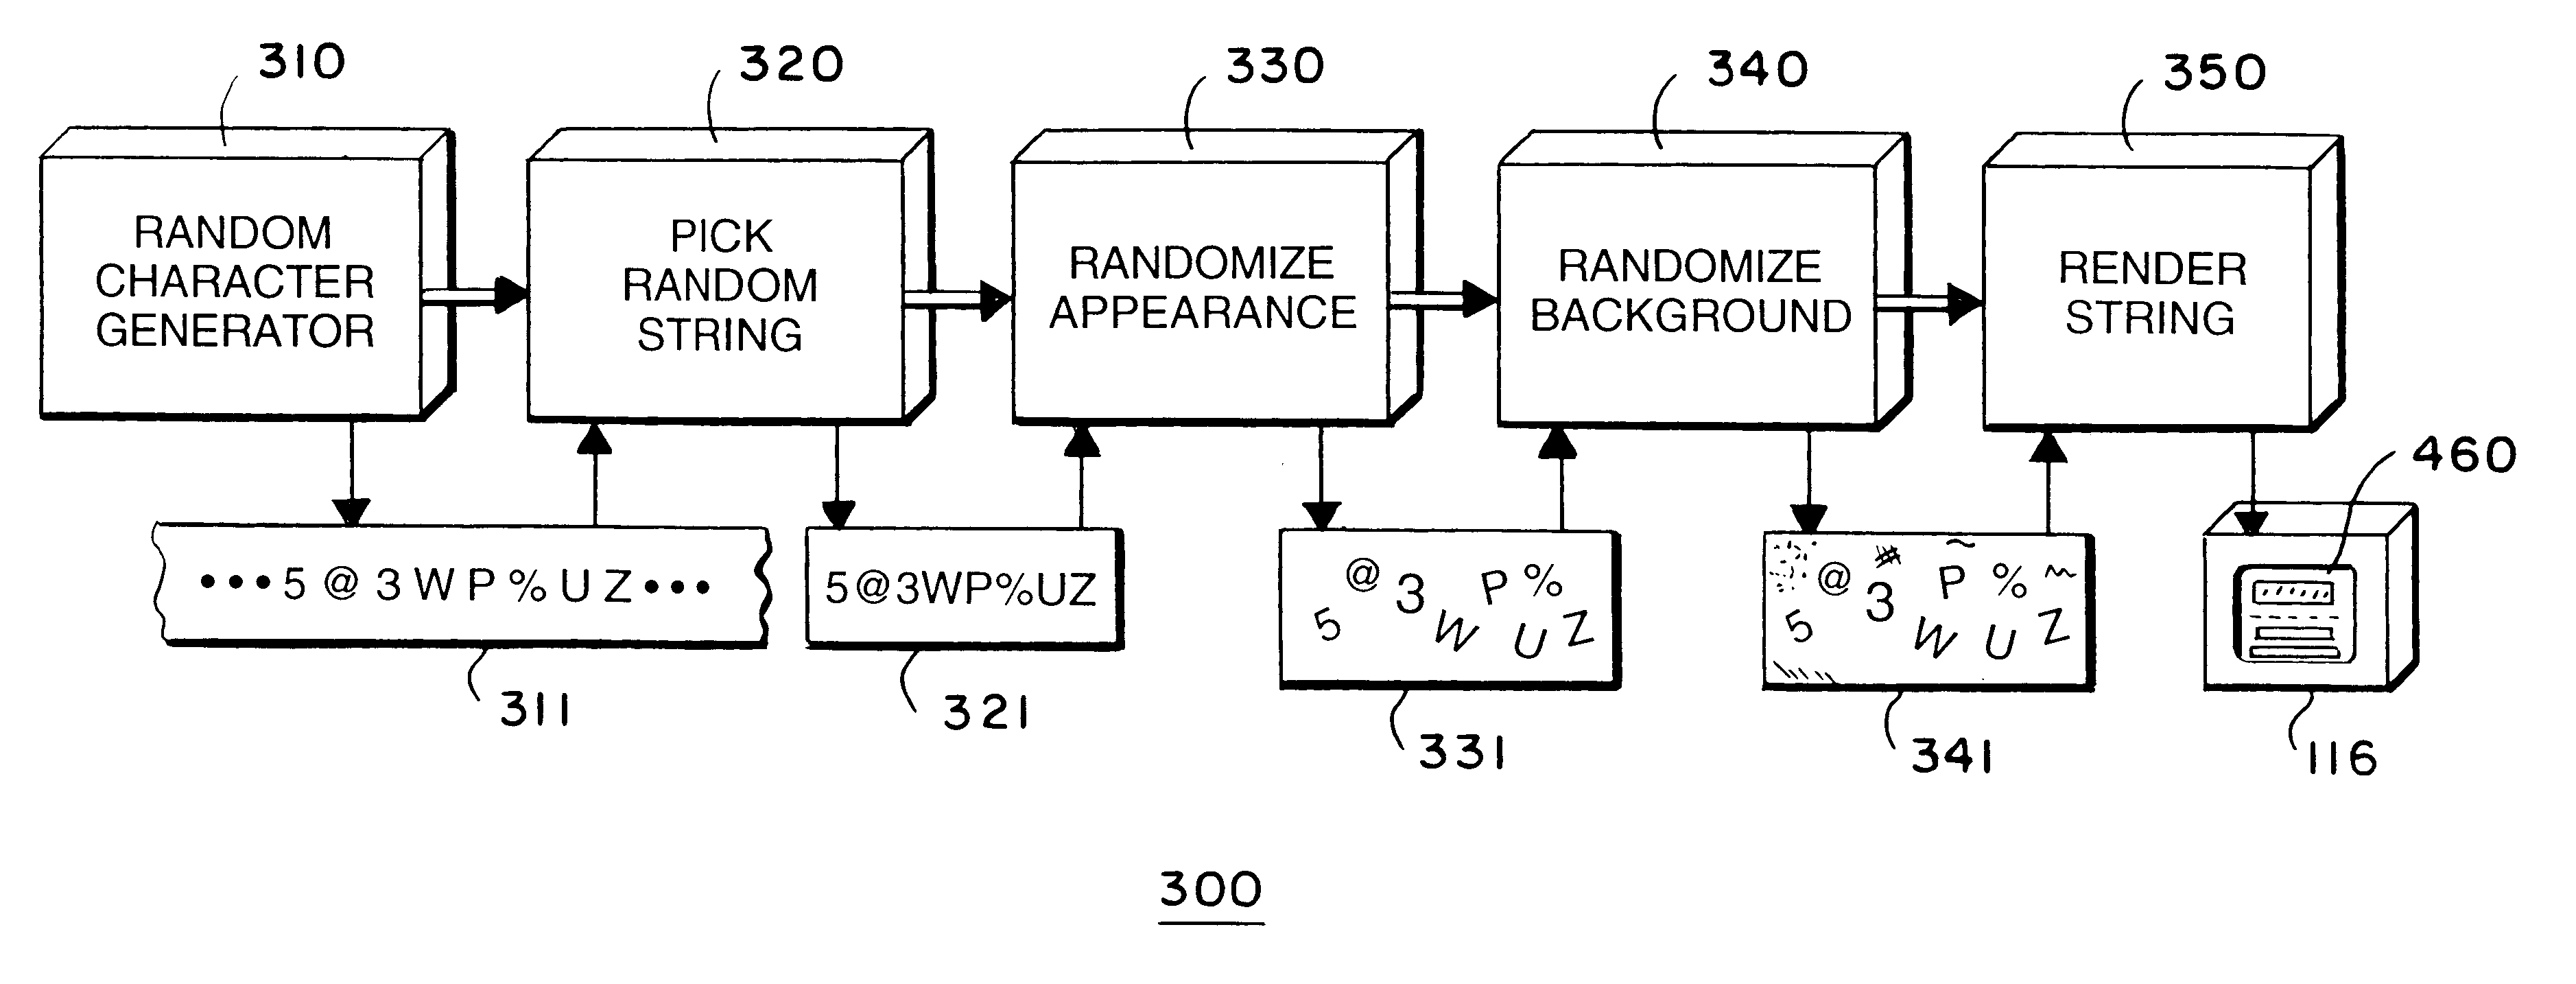
\includegraphics[width=0.49\textwidth]{img01.png}
	\caption{Text-based CAPTCHA generation as described by Lillibridge et al}
	\label{fig:img01}
\end{figure}

\indent Nowadays, there are several variations of CAPTCHAs apart from the original text-based CAPTCHA \cite{jeng10}. Examples of such tests are audio-based tests, image-based tests such as identifying images that satisfy certain conditions, and video-based tests such as recognizing objects and/or text from a video. Regardless, text-based CAPTCHAs are still used because they are easily recognizable by humans, they are easy to generate, and because image and video-based CAPTCHAs require large databases of images/videos because reusing the same images/videos may make the system prone to hacking.\\

\indent Solving a text-based CAPTCHA can be broken down into the following steps \cite{bursztein11}:
\begin{itemize}[\topsep=0pt]
  \item The \textbf{preprocessing} step involves the removal of backgrounds, lines, and other types of noise that may affect the solving of the CAPTCHA.
  \item The \textbf{segmentation} step is the separation of the text image into individual character images.
  \item The \textbf{post-processing} step is an optional step that cleans up or improves the segmentation output. An example of a process done in this step is the normalization of the sizes of output character images.
  \item The \textbf{recognition} step is the identification of the characters corresponding to the character images.
\end{itemize} 
Since computers can beat humans in recognizing single characters including distortions \cite{chellapilla05}, it is important for a text-based CAPTCHA image to be hard to segment into individual characters. CAPTCHA generators do this by applying anti-segmentation techniques \cite{bursztein11} such as applying complex backgrounds, occluding lines, and negative kerning or reducing the space between letters. Anti-recognition techniques such as using multiple fonts, different character sets, variable font sizes, character distortion or blurring, character tilting, and word waving are also applied to the text image to make computer recognition even harder.\\

\indent [INSERT RELATED WORK HERE] \\

\indent This project aims to study the performance of various machine learning classifiers on the solving of text-based CAPTCHAs. In particular, it aims to identify how many CAPTCHAs can be solved depending on the machine learning algorithm, the per-letter accuracy of each algorithm, and the time it takes for each algorithm to answer a CAPTCHA.

% An example of a floating figure using the graphicx package.
% Note that \label must occur AFTER (or within) \caption.
% For figures, \caption should occur after the \includegraphics.
% Note that IEEEtran v1.7 and later has special internal code that
% is designed to preserve the operation of \label within \caption
% even when the captionsoff option is in effect. However, because
% of issues like this, it may be the safest practice to put all your
% \label just after \caption rather than within \caption{}.
%
% Reminder: the "draftcls" or "draftclsnofoot", not "draft", class
% option should be used if it is desired that the figures are to be
% displayed while in draft mode.
%
%\begin{figure}[!t]
%\centering
%\includegraphics[width=2.5in]{myfigure}
% where an .eps filename suffix will be assumed under latex, 
% and a .pdf suffix will be assumed for pdflatex; or what has been declared
% via \DeclareGraphicsExtensions.
%\caption{Simulation results for the network.}
%\label{fig_sim}
%\end{figure}

% Note that the IEEE typically puts floats only at the top, even when this
% results in a large percentage of a column being occupied by floats.

\section{Review of Related Literature}
\subsection{Morphology}
Digital image processing is the application of algorithms to an image represented as a set of pixels mapped to a two-dimensional area for purposes such as classifying the image or extracting important features from it. Examples of operations used to process images are \textbf{morphological operations}. Mathematical morphology \cite{serra83} is the processing of geometric structures using concepts from set theory. In image processing, it is the combination of an image and a structuring element using set operations such as union and intersection to generate a new image. Since morphological operators are extensively used in binary (i.e. black and white) images, the first step of morphology in image processing is usually the conversion of a colored or a grayscale image to a binary image; this is called thresholding. A thresholding operation is defined as
\[ \theta(f,t) = 
   \begin{cases} 
    1 & f\geq t \\
    0 & \text{otherwise} \\
   \end{cases}
\]
where f is the function value resulting from some sort of thresholding method, and 1 \& 0 are foreground and background values, respectively. Thresholding methods can be based on histogram shape, gray-level clustering, entropy of foreground and background regions, similarity measures between attributes such as edges, and so on \cite{sezgin04}.\\

\indent In digital image processing, the structuring element is a convolution matrix consisting of 1's and 0's, which is also called a kernel. The most basic morphological operations are erosion and dilation \cite{fisher03}. For both of these operations, the kernel is first superimposed on top of each pixel and its neighbors such that the center of the kernel is superimposed on top of the pixel itself. Depending on the operation, the new value of each pixel is as follows:
\begin{itemize}[\topsep=0pt]
  \item For \textbf{erosion}, if at least one 1-value on the kernel is superimposed on top of a 0-valued image pixel, the new pixel value is 0. Otherwise, it is 1.
  \item For \textbf{dilation}, if at least one 1-value on the kernel is superimposed on top of a 1-valued image pixel, the new pixel value is 1. Otherwise, it is 0.
\end{itemize} 
\begin{figure}[h]
	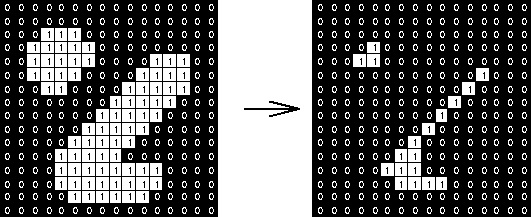
\includegraphics[width=0.49\textwidth]{erodbin.jpg}
	\caption{Example of an erosion operation}
	\label{fig:erodbin}
\end{figure}
Kernels can be of different shapes; for example, a square kernel is one whose elements are all 1's while a cross kernel is one whose 1's are on the middle row and middle column only. \hyperref[fig:erodbin]{\autoref{fig:erodbin}} shows the result of the erosion of an image using a $3 \times 3$ square kernel. In general, erosion is used to shrink foreground regions and enlarge holes, while dilation is used to enlarge foreground regions and shrink holes. Other operations include opening and closing, top-hat and black-hat transforms, and the morphological gradient.

\subsection{K-means clustering}
Clustering is the grouping of a set of objects so that the objects in a group are similar to one another and objects from different groups are different from one another [REF?]. From a mathematical perspective, the goal of clustering is to minimize the intra-cluster distance, a measure of dissimilarity between elements in a cluster, and to maximize the inter-cluster distance, a measure of dissimilarity between different clusters. Clusters can be formed using different types of algorithms; examples of these are hierarchical or connectivity-based algorithms such as SLINK \cite{sibson73}, density-based algorithms such as DBSCAN \cite{ester96}, and centroid-based algorithms such as k-means \cite{lloyd82}.\\

The k-means clustering algorithm clusters a data set based on the number of clusters specified beforehand. Random points as many as the number of clusters are selected from either the data set or the data domain, and these points shall serve as "means" for the initial clustering. Each point is assigned to a cluster whose "mean" is closest to it. After all the points are assigned, the centroids (the geometric means of the cluster points) are computed and will then serve as means for the next clustering iteration. The assignment of points to clusters and selection of new means are done iteratively until convergence is reached, which is when the resulting clusters of an iteration are the same as the clusters in its previous iteration . An illustration of the algorithm is shown by \hyperref[fig:kmean]{\autoref{fig:kmean}}.
\begin{figure}[htbp]
        \begin{subfigure}{0.23\textwidth}
                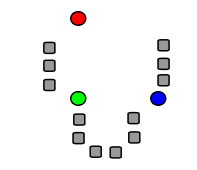
\includegraphics[width=\textwidth]{kmean01.png}
                \caption{Selection of initial means}
                \label{fig:kmean01}
        \end{subfigure}
        \begin{subfigure}{0.23\textwidth}
                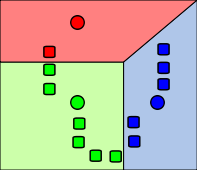
\includegraphics[width=\textwidth]{kmean02.png}
                \caption{Creation of clusters}
                \label{fig:kmean02}
        \end{subfigure}
        \begin{subfigure}{0.23\textwidth}
                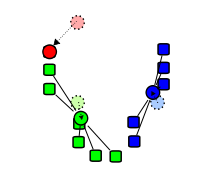
\includegraphics[width=\textwidth]{kmean03.png}
                \caption{Computation of centroids}
                \label{fig:kmean03}
        \end{subfigure}
        \begin{subfigure}{0.23\textwidth}
                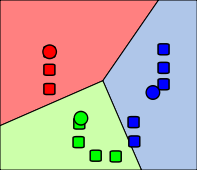
\includegraphics[width=\textwidth]{kmean04.png}
                \caption{Cluster reconfiguration}
                \label{fig:kmean04}
        \end{subfigure}
        \caption{Illustration of the K-means algorithm (by Weston Pace, distributed under a CC BY-SA 3.0 license)}
        \label{fig:kmean}
\end{figure}
\subsection{Machine Learning and Classification}

Machine learning is the science of giving computers the ability to progressively improve their performance on processing data without being explicitly programmed \cite{samuel59}. It involves the construction of algorithms that can learn from data to make predictions on other data of the same nature. Machine learning has several applications, which include spam filtering \cite{guzella09}, medical imaging \cite{wernick10}, and intruder detection on computer networks \cite{sommer10}. In general, machine learning is used for tasks such as classification, regression, dimensionality reduction, density estimation, clustering, and so on.

\indent Classification is the identification of the class of a new observation based on its quantifiable properties or features and the information derived from a training set of data whose classes are known [REF?]. Algorithms that perform the mapping of data to classes are called classifiers. Classifiers have different approaches to classifying data, some of which are described below.

\subsubsection{K-Nearest Neighbor}
The k-nearest neighbor classifier \cite{altman92} is an instance-based learning algorithm that assigns a class to an observation based on the classes of the training data that are closest to it with respect to some similarity measure. Suppose there exist an observation $X_t$ with an unknown class and pairs $(X_1,Y_1),(X_2,Y_2),...,(X_n,Y_n)$ where $X_i$ and $Y_i$ are the i\textsuperscript{th} training datum and its corresponding label, respectively. Let $(X_{(1)},Y_{(1)}),(X_{(2)},Y_{(2)}),...,(X_{(n)},Y_{(n)})$ be a sequence of order statistics such that  $\lvert\lvert (X_{(1)}-X_t) \rvert\rvert \leq \lvert\lvert (X_{(2)}-X_t) \rvert\rvert \leq ... \leq \lvert\lvert (X_{(n)}-X_t) \rvert\rvert$. The class of $X_t$ is defined as
\[ Y_t = \text{mode}(Y_{(1)},Y_{(2)},...,Y_{(k)})\]
where $Y_{(i)}$ is the class of the order statistic $X_{(i)}$ and $k$ is a user-defined, preferably odd positive integer that indicates the number of nearest neighbors to be considered for classification. In case of ties in classification, $k$ is decremented by 1 until the tie is resolved. For example, if applying the k-NN algorithm on an observation with $k = 5$ results into labels $(1,2,1,2,4)$, $k$ will be reduced to 3 to break the tie and the observation will be given the label 1. 
\subsubsection{Support Vector Machines}
A support vector machine \cite{cortes95} is a classifier that identifies the hyperplane that separates two sets of data with the highest margin of separation. More formally, [DISCUSS FORMULA HERE; ALSO, BRIEFLY STATE HARD/SOFT MARGIN and KERNEL TRICKS]
\subsubsection{Random Forest}

\subsubsection{Deep Learnin}
% An example of a double column floating figure using two subfigures.
% (The subfig.sty package must be loaded for this to work.)
% The subfigure \label commands are set within each subfloat command,
% and the \label for the overall figure must come after \caption.
% \hfil is used as a separator to get equal spacing.
% Watch out that the combined width of all the subfigures on a 
% line do not exceed the text width or a line break will occur.
%
%\begin{figure*}[!t]
%\centering
%\subfloat[Case I]{\includegraphics[width=2.5in]{box}%
%\label{fig_first_case}}
%\hfil
%\subfloat[Case II]{\includegraphics[width=2.5in]{box}%
%\label{fig_second_case}}
%\caption{Simulation results for the network.}
%\label{fig_sim}
%\end{figure*}
%
% Note that often IEEE papers with subfigures do not employ subfigure
% captions (using the optional argument to \subfloat[]), but instead will
% reference/describe all of them (a), (b), etc., within the main caption.
% Be aware that for subfig.sty to generate the (a), (b), etc., subfigure
% labels, the optional argument to \subfloat must be present. If a
% subcaption is not desired, just leave its contents blank,
% e.g., \subfloat[].


% An example of a floating table. Note that, for IEEE style tables, the
% \caption command should come BEFORE the table and, given that table
% captions serve much like titles, are usually capitalized except for words
% such as a, an, and, as, at, but, by, for, in, nor, of, on, or, the, to
% and up, which are usually not capitalized unless they are the first or
% last word of the caption. Table text will default to \footnotesize as
% the IEEE normally uses this smaller font for tables.
% The \label must come after \caption as always.
%
%\begin{table}[!t]
%% increase table row spacing, adjust to taste
%\renewcommand{\arraystretch}{1.3}
% if using array.sty, it might be a good idea to tweak the value of
% \extrarowheight as needed to properly center the text within the cells
%\caption{An Example of a Table}
%\label{table_example}
%\centering
%% Some packages, such as MDW tools, offer better commands for making tables
%% than the plain LaTeX2e tabular which is used here.
%\begin{tabular}{|c||c|}
%\hline
%One & Two\\
%\hline
%Three & Four\\
%\hline
%\end{tabular}
%\end{table}


% Note that the IEEE does not put floats in the very first column
% - or typically anywhere on the first page for that matter. Also,
% in-text middle ("here") positioning is typically not used, but it
% is allowed and encouraged for Computer Society conferences (but
% not Computer Society journals). Most IEEE journals/conferences use
% top floats exclusively. 
% Note that, LaTeX2e, unlike IEEE journals/conferences, places
% footnotes above bottom floats. This can be corrected via the
% \fnbelowfloat command of the stfloats package.
\section{Methodology}
[OTSU, OPENING, KMEANS, CLASSIFIER]
\subsection{Preprocessing}
\subsection{Segmentation and Post-processing}
\subsection{Recognition}
\section{Results and Discussion}
\subsection{Experiment specifications}
\subsection{Experiment results}

\section{Conclusion}
The conclusion goes here.




% conference papers do not normally have an appendix



% use section* for acknowledgment
%\ifCLASSOPTIONcompsoc
  % The Computer Society usually uses the plural form
 % \section*{Acknowledgments}
%\else
  % regular IEEE prefers the singular form
 % \section*{Acknowledgment}
%\fi




% trigger a \newpage just before the given reference
% number - used to balance the columns on the last page
% adjust value as needed - may need to be readjusted if
% the document is modified later
%\IEEEtriggeratref{8}
% The "triggered" command can be changed if desired:
%\IEEEtriggercmd{\enlargethispage{-5in}}

% references section

% can use a bibliography generated by BibTeX as a .bbl file
% BibTeX documentation can be easily obtained at:
% http://mirror.ctan.org/biblio/bibtex/contrib/doc/
% The IEEEtran BibTeX style support page is at:
% http://www.michaelshell.org/tex/ieeetran/bibtex/
%\bibliographystyle{IEEEtran}
% argument is your BibTeX string definitions and bibliography database(s)
%\bibliography{IEEEabrv,../bib/paper}
%
% <OR> manually copy in the resultant .bbl file
% set second argument of \begin to the number of references
% (used to reserve space for the reference number labels box)
% \begin{thebibliography}{1}

\bibliographystyle{IEEEtran}
\bibliography{refs}
% \end{thebibliography}




% that's all folks
\end{document}


